\documentclass[12pt]{article}
\usepackage{alltt}
\usepackage[utf8]{inputenc}
\usepackage[dvips]{graphicx}
%\usepackage{a4wide}
\usepackage{epsfig}
\usepackage{fancybox}
\usepackage{verbatim}
\usepackage{array}
\usepackage{latexsym}
\usepackage{alltt}
%\usepackage{dsfont}
\usepackage{caption}
\usepackage{subcaption}
%\usepackage{fullpage}
\usepackage{hyperref}
\usepackage{textcomp}
\usepackage{listings}
\usepackage{color}
\usepackage{amsmath}
\usepackage{amsfonts}
\usepackage{tikz}
\usepackage{float}
\usepackage{matlab-prettifier}
\usepackage{graphicx}

\usepackage[hmargin=3cm,vmargin=6.0cm]{geometry}
%\topmargin=0cm
\topmargin=-2cm
\addtolength{\textheight}{6.5cm}
\addtolength{\textwidth}{2.0cm}
%\setlength{\leftmargin}{-5cm}
\setlength{\oddsidemargin}{0.0cm}
\setlength{\evensidemargin}{0.0cm}

%misc libraries goes here

\begin{document}

\section*{Student Information } 
%Write your full name and id number between the colon and newline
%Put one empty space character after colon and before newline
Full Name :  Doruk Berke Yurtsizoglu\\
Id Number :  2522225\\

% Write your answers below the section tags
\section*{Answer 1}

\subsection*{a)} 
Variables are discrete from each other. Therefore, we will use the equation $E(x) = \sum x*f(x)$ .\\
\\
For blue dice:\\
$E(x) = \sum x*f(x) = 1*1/6 + 2*1/6 + 3*1/6 + 4*1/6 + 5*1/6 + 6*1/6 = 3.5$\\
For yellow dice:\\
$E(x) = \sum x*f(x) = 1*3/8 + 3*3/8 + 4*1/8 + 8*1/8 = 3$\\
For red dice:\\
$E(x) = \sum x*f(x) = 2*5/10 + 3*2/10 + 4*2/10 + 6*1/10 = 3$\\

\subsection*{b)} 
I would choose the 3 blue dice option since the sum of expected values of that option is greater than the other choice.\\
Three blue dice: $3.5+3.5+3.5 = 10.5$\\
A single dice from each color: $3.5 + 3 + 3 = 9.5$\\

\subsection*{c)} 
I would choose a single die of each color because this time the expected value of the yellow die becomes 8 which makes the single die of each color option's expected value greater.\\
Three blue dice: $3.5+3.5+3.5 = 10.5$\\
A single dice from each color: $3.5 + 8 + 3 = 14.5$\\

\subsection*{d)} 
$T \rightarrow$ getting three as result\\
$R \rightarrow$ the dice is red\\
\\
$P(R|T) = \dfrac{P(T|R)*P(R)}{P(T|R)*P(R) + P(T|\overline R)*P(\overline R)}$\\
\\
$P(R) = 1/3$, $P(\overline R) = 2/3$, $P(T|R) = 2/10 = 1/5$, $P(T|\overline R) = 1/2*1/6+1/2*3/8 = 13/48$\\
\\
$P(R|T) = \dfrac{1/5*1/3}{1/5*1/3 + 13/48*2/3}$\\
\\
$P(R|T) = 0.2696$\\


\subsection*{e)} 
When we roll blue and yellow dice together, the number of possible outcomes will be 48.(6*8)\\
Combinations of getting a total value of 5 are:\\

\begin{table}[H]
        \centering
        \begin{tabular}{|c|c|c|}
		\hline
		Blue Dice & Yellow Dice & Possibility\\
		\hline
		1 & 4 & 1/6*1/8 = 1/48\\
		4 & 1 & 1/6*3/8 = 3/48\\
		2 & 3 & 1/6*3/8 = 3/48\\
		3 & 2 & 1/6*0 = 0\\
		\hline
               
        \end{tabular}
        

    \end{table}{}

The result is 1/48 + 3/48 + 3/48 + 0 = 7/48 = 0.146\\

\section*{Answer 2}

\subsection*{a)} 
Normally, this is a binomial distribution question because days are independent from each other. However, it is better to us poisson approximation to binomial because n = 80 $\geq$ 10, and p = 0.025 $\leq$ 0.05. The equation which leads to this approximation is $\lambda = n*p$. Moreover, the poisson distribution is $P(X=x) = \dfrac{e^{-\lambda}*\lambda^{x}}{x!}$.\\
\\
p = possibity for A to make a discount on a specific day = 0.025\\
n = 80\\
$\lambda$ = n*p = 80*0.025 = 2\\
At least 4 $\implies$ $P(X \geq 4) = 1 - F(3)$\\
$P(X \geq 4) = 1 - F(3)$\\
$P(X \geq 4) = 1 - \dfrac{e^{-2}*2^{3}}{3!} - \dfrac{e^{-2}*2^{2}}{2!} - \dfrac{e^{-2}*2^{1}}{1!} -\dfrac{e^{-2}*2^{0}}{0!}$\\
\\

$P(X \geq 4) = 1 - 0.8578 = 0.1428$\\



\subsection*{b)} 
Let A: A makes a discount,\\
Let B: B makes a discount.\\
In order to buy a telephone, A or B must make a discount.\\
P(A or B) = 1 - P(not A and not B)\\
Probability of A to not make a discount = $\binom{80}{0}*(0.025)^0*(0.975)^80$ = 0.131\\
Probability of B to not make a discount = $\binom{1}{0}*(0.1)^0*(0.9)^1$ = 0.9\\
\\
Probability of not making a discount in 2 days for A and B:\\
$-$ A doen't make a discount on day 1.\\
$-$ A doen't make a discount on day 2.\\
$-$ B doen't make a discount on both days.\\
Then, Probability of not making a discount in 2 days for A and B = (0.131)*(0.131)*(0.9)*(0.9) = 0.139\\
P(A or B) = 1 - 0.139 = 0.986\\

\section*{Answer 3}

\begin{lstlisting}[style=Matlab-editor]

%%My Code
roll_dice_and_plot()
roll_dice_1000_times()

function []= roll_dice_1000_times()
    count = 0
    b_dice = randsample([1 2 3 4 5 6], 1000, true, [1/6 1/6 1/6 1/6 1/6 1/6])
    y_dice = randsample([1 3 4 8], 1000, true, [3/8 3/8 1/8 1/8])
    r_dice = randsample([2 3 4 6], 1000, true, [5/10 2/10 2/10 1/10])

    first_opt = [b_dice + y_dice + r_dice]
    second_opt = [b_dice + b_dice + b_dice]

    for n = 1:length(first_opt)
        if second_opt(n) > first_opt(n) 
            count = count + 1
        end
    end
    per = count/1000
    disp(['Percentage of the cases where the total value of the second option is greater than the first option is ',num2str(per)])

end



function []= roll_dice_and_plot()
    
    N = 1000
    b_dice = randsample([1 2 3 4 5 6], N, true, [1/6 1/6 1/6 1/6 1/6 1/6])
    y_dice = randsample([1 3 4 8], N, true, [3/8 3/8 1/8 1/8])
    r_dice = randsample([2 3 4 6], N, true, [5/10 2/10 2/10 1/10])
    
    av_val_op1 = sum(b_dice + y_dice + r_dice)/(N)
    av_val_op2 = sum(b_dice + b_dice + b_dice)/(N)
    
    if av_val_op1 > av_val_op2
        disp('Rolling a single die of each color is preferrable.')
    
    elseif av_val_op2 > av_val_op1
        disp('Rolling three blue dice is preferrable.')
        

    else
        roll_dice()
    end

    figure
        histogram(b_dice,FaceColor="b");
        xlim([1, 10]);
        xlabel('Rolling Result', 'FontSize', 14);
        ylabel('Occurrence', 'FontSize', 14);
        title('Histogram for Blue Dice')
        
        figure
        histogram(y_dice,FaceColor="y");
        xlim([1, 10]);
        xlabel('Rolling Result', 'FontSize', 14);
        ylabel('Occurrence', 'FontSize', 14);
        title('Histogram for Yellow Dice')
        
        figure
        histogram(r_dice,FaceColor="r");
        xlim([1, 10]);
        xlabel('Rolling Result', 'FontSize', 14);
        ylabel('Occurence', 'FontSize', 14);
        title('Histogram for Red Dice')
end
\end{lstlisting}

\begin{figure}[h!]
  \centering
  \begin{subfigure}[b]{0.4\linewidth}
    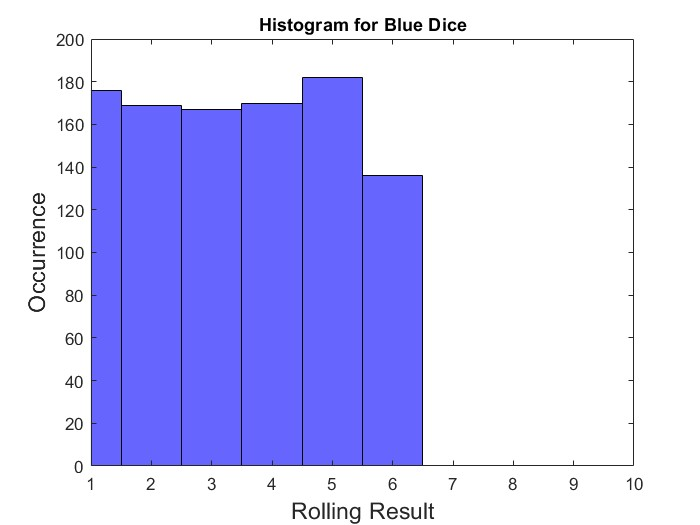
\includegraphics[width=\linewidth]{blue.jpg}
    \caption{Blue Dice}
  \end{subfigure}
  \begin{subfigure}[b]{0.4\linewidth}
    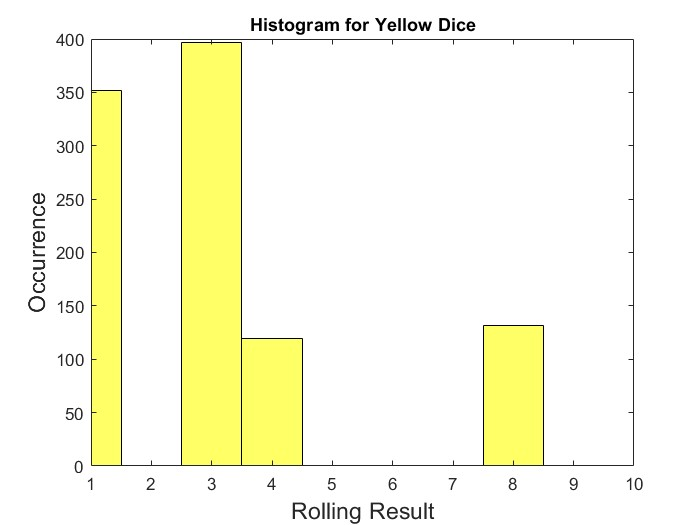
\includegraphics[width=\linewidth]{yellow.jpg}
    \caption{Yellow Dice}
  \end{subfigure}
  \begin{subfigure}[b]{0.4\linewidth}
    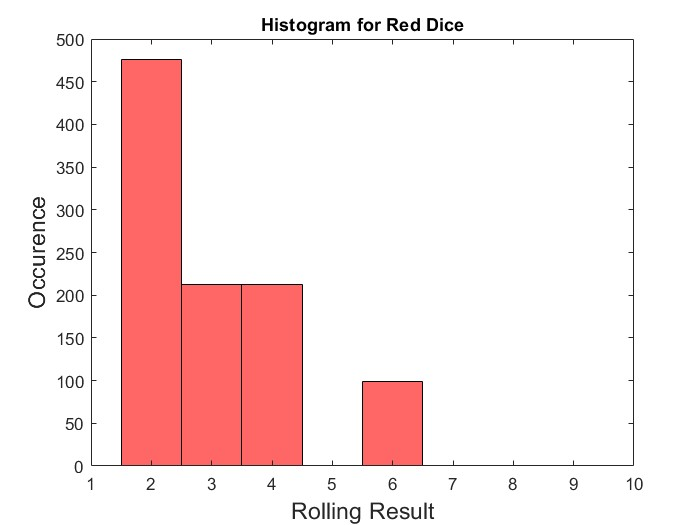
\includegraphics[width=\linewidth]{red.jpg}
    \caption{Red Dice}
   \end{subfigure}
  \caption{Graphs of Results}
  \label{fig:coffee}
\end{figure}

\begin{figure}[h!]
  \centering
  \begin{subfigure}[b]{0.4\linewidth}
    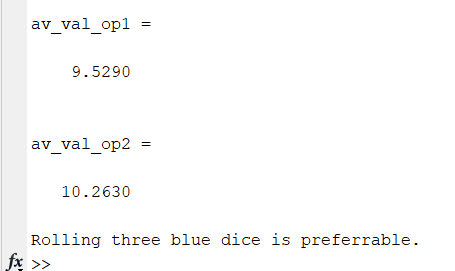
\includegraphics[width=\linewidth]{print.jpg}
    \caption{Printed Result of the Experiment}
  \end{subfigure}
  \begin{subfigure}[b]{0.4\linewidth}
   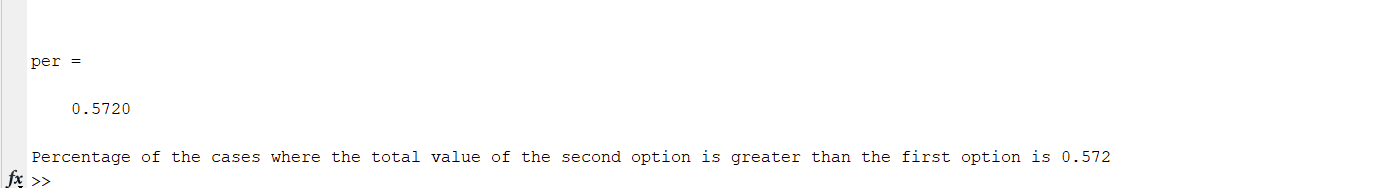
\includegraphics[width=\linewidth]{avg.png}
   \caption{Printed Result of Percentage of Option 2 Wins}
  \end{subfigure}
\end{figure}




\end{document}